\section{Электромагнитные волны на границе раздела двух диэлектриков. Зависимость коэффициентов отражения от угла падения (качественно). Явление Брюстера.}
\subsection{Электромагнитные волны на границе раздела двух диэлектриков. }
На границе мы можем выделить 2 коэффициента: отражения и пропускания $r$ и $t$. Ну и там дальше душная френелевская хуйня.
\subsection{Зависимость коэффициентов отражения от угла падения (качественно). Явление Брюстера.}
На рисунке показана зависимость коэффициента отражения $R(\theta)$ для $s$-поляризованного ($R_{\perp}$) и $p$-поляризованного ($R_{\parallel}$) излучения.\\
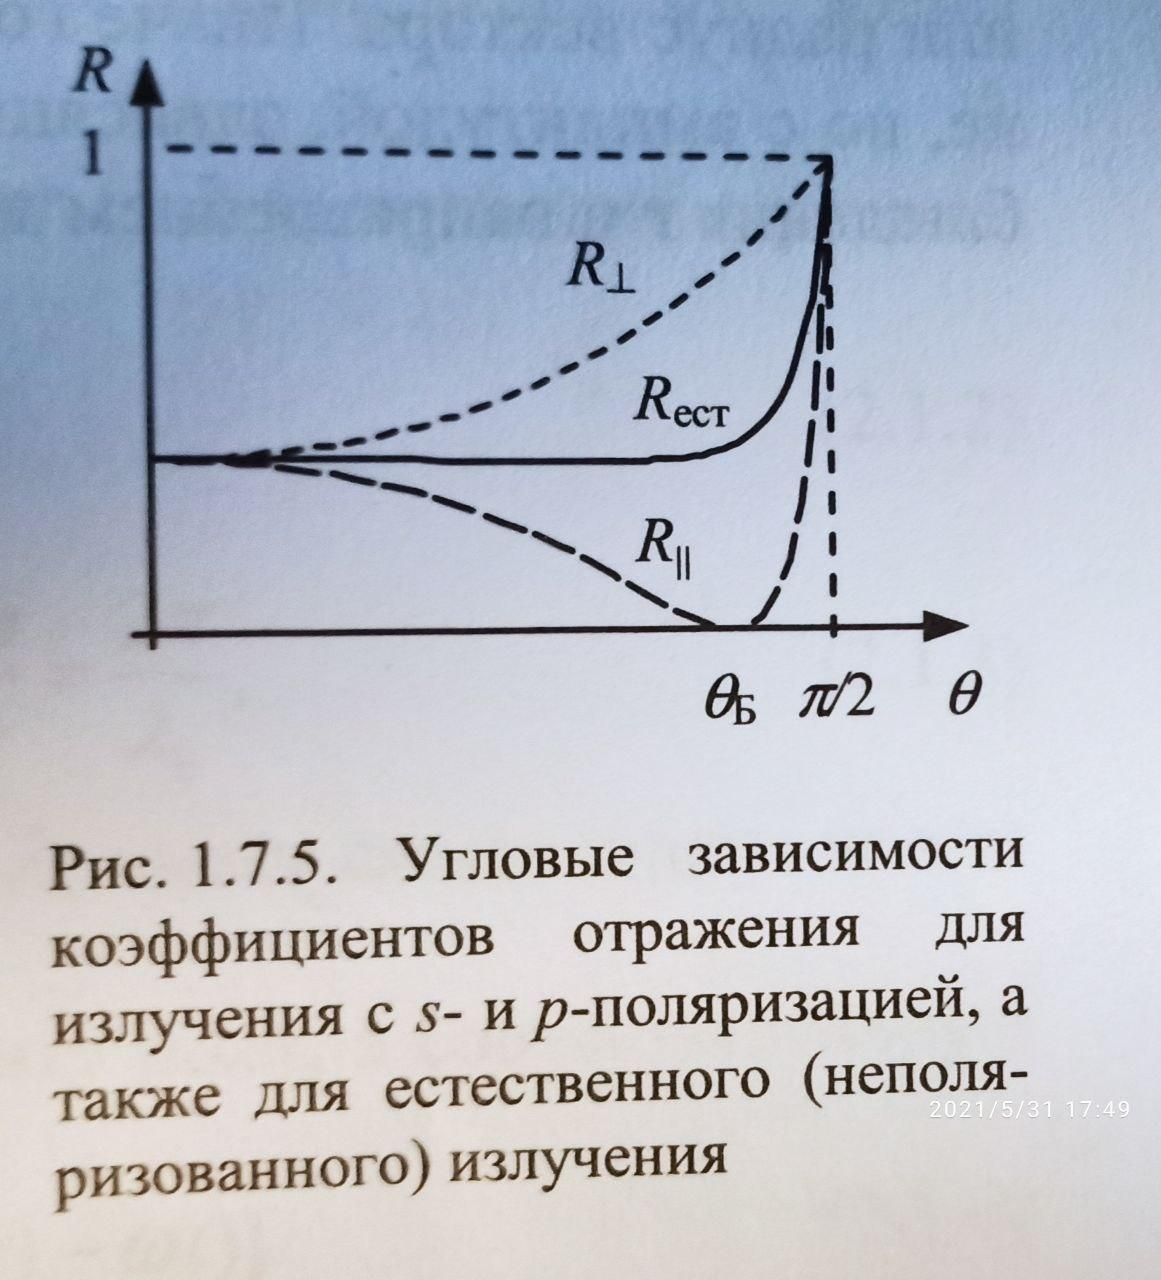
\includegraphics[width=\textwidth]{parts/img/p5_kach.jpg}\\
В случае $p$-поляризованной волны существует такой угол $\theta = \theta_Б$, называемый углом Брюстера, что волна падающая под этим углом на поверхность не отражается обратно. Полагая в формулах Френеля $r_{\parallel}(\theta) = 0$, этот угол будет
$$\operatorname{tg} \theta_Б = n_2/n_1$$
При падении под углом брюстера отражённая волна становится полностью $s$-поляризованной.
